\documentclass{article}

% Language setting
% Replace `english' with e.g. `spanish' to change the document language
\usepackage[french]{babel}

% Set page size and margins
% Replace `letterpaper' with `a4paper' for UK/EU standard size
\usepackage[letterpaper,top=2cm,bottom=2cm,left=3cm,right=3cm,marginparwidth=1.75cm]{geometry}

% Useful packages
\usepackage{amsmath}
\usepackage{graphicx}
\usepackage[colorlinks=true, allcolors=blue]{hyperref}
\usepackage{mathtools,amssymb}
\usepackage{caption}
\usepackage{subcaption}
\usepackage{lipsum} 
\usepackage{adjustbox}
\usepackage{pgffor}
\title{Learning Active Contour Models for Medical Image Segmentation}
\author{Nissim Maruani}

\begin{document}

\newcommand{\animage}[1][example-image]{\adjustbox{valign=m,vspace=2pt}{\includegraphics[width=.24\linewidth]{#1}}}

\maketitle
 
\section{Étude synthétique de l'article}


\subsection{Problème traité}

L'article étudié \cite{learningcontour} s'attaque au problème de segmentation dans une image, appliqué ici au milieu médical. Les images concernées sont des IRM du cœur dont il faut segmenter trois régions : le ventricule droit, le ventricule gauche et le myocarde. La détection de ces régions est un enjeu fondamental puisqu'elle permet au praticien de prévenir ou d'identifier des maladies cardiovasculaires qui tuent chaque année 17.9 millions de personnes. La segmentation consiste à partir d'une image $u \in \mathbb{R}^{H \times W \times d}$ (de dimension $d=3$ pour une image en couleur RGB, $d=1$ pour une image en niveau de gris) à produire une image segmentée $v \in \{0... k-1\}^{H \times W}$ où chaque pixel peut appartenir à $k$ régions différentes. 

\subsection{Méthodes utilisées et originalité de l'article}

Pour segmenter ces trois régions, l'article propose d'utiliser des réseaux de neurones convolutifs (aussi appelés CNN). Les convolutions, invariantes par translations, sont très utilisées dans l'analyse d'images : associées à des fonctions d'activations non linéaires (ici $ReLU(x) = \max(x, 0)$) et à des sous échantillonnages à différentes échelles (MaxPool), elles permettent de modéliser efficacement des phénomènes complexes. \\

Pour entraîner ces réseaux de neurones, on utilise ici des images IRM segmentées précisément par des humains : on calcule l'erreur (en anglais \textit{loss}) entre la segmentation prédite par l'algorithme et celle exacte puis l'on modifie les poids des convolutions par une descente de gradient (en anglais \textit{back-propagation}). Des nouvelles images (qui n'ont pas été vues par le réseau pendant la phase d'entraînement) permettent de mesurer les performances de l'algorithme.\\

L'article étudié propose d'utiliser une structure classique de réseau convolutif appelé U-Net \cite{unet}. Chacune des trois régions est segmentée par un réseau différent. L'output de chaque réseau est donc une image en niveau de gris  $y_{pred}  \in [0,1]^{H \times W}$ qui nous permet d'obtenir la segmentation prédite $1_{y_{pred}>0.5} \in \{0,1\}^{H \times W}$. Pour les problèmes de classification, la loss la plus classique est la \textit{Cross Entropy Loss}, définie par : 
\[ CE(y_{pred},y_{true}) = - \frac{1}{H \times W} \sum_{i,j} y_{true}(i,j) \log{(y_{pred}(i,j))} + (1-y_{true}(i,j))  \log{(1-y_{pred}(i,j))} \]

L'originalité de l'article est de proposer une fonction de perte inspirée des contours actifs qui prend en compte non seulement le label des régions, mais aussi la longueur de la bordure, à savoir :
\[ L(y_{pred}) = \sum_{i,j} \sqrt{ \vartriangle_h y_{pred}(i,j)^2 + \vartriangle_v y_{pred}(i,j)^2  } \ \textnormal{avec} \ \left \{
\begin{array}{c @{=} c}
    \vartriangle_h u(i,j) & u(i+1,j) - u(i,j)   \\
    \vartriangle_v u(i,j) & u(i,j+1) - u(i,j)  
\end{array}
\right. \]

Pour obtenir la loss AC suivante, paramétrée par $\lambda \in \mathbb{R}$:
 \[ AC(y_{pred},y_{true})  =  L(y_{pred}) + \lambda \sum_{i,j} y_{true}(i,j) (1-y_{pred}(i,j))^2 +  (1-y_{true}(i,j)) y_{pred}(i,j)^2 \]
 
Pour mesurer les performances de l'algorithme, deux métriques sont utilisées, le \textit{Dice Score} et la distance de Hausdorff. Le calcul du \textit{Dice Score} est le suivant :

 \[ DC(y_{pred},y_{true})  =  2 \frac{\sum_{i,j} y_{true}(i,j) y_{pred}(i,j)}{\sum_{i,j} y_{true}(i,j) + y_{pred}(i,j)}  \]
 
La distance de Hausdorff mesure la distance entre deux segmentations. Dans un cadre général, pour deux ensembles de points $A$ and $B$, la distance de Hausdorff est définie par :
\[ H(A,B) = max(h(A,B), h(B,A)) \ \textnormal{avec}  \]

\[ h(A,B) = \max_{a \in A} \min_{b \in B} ||a-b||_2\]

\subsection{Comparaison au cours}

Nous avons vu en cours des approches classiques (sans apprentissage) permettant de segmenter des formes \cite{findingclosed} \cite{brainseg} \cite{finsler} \cite{globalmin}. Ces approches fonctionnent également à l'aide de la minimisation d'une énergie : c'est d'ailleurs l'une d'entre elles \cite{globalmin} qui a inspiré la loss AC utilisée dans l'article. Ces approches classiques sont cependant plus susceptibles de rester coincées dans un minimum local. Elles sont également plus lentes, puisque la descente de gradient est faite individuellement sur chaque image. De plus, l'initialisation de ces contours actifs est un problème non trivial, et l'on souhaite ici se passer d'un input de l'utilisateur : un réseau de neurone ne requiert aucune autre information que l'image pour segmenter les sections cherchées. 


\subsection{Nouveaux résultats}

Les résultats annoncés dans l'article surpassent l'état de l'art. Avec la nouvelle métrique, la distance de Hausdorff obtenue est $40\%$ meilleure et le Dice Score passe de $95\%$ à $98.6\%$ sur ce problème de segmentation.

\subsection{Avis critique}

Une lecture approfondie de l'article soulève plusieurs questions. La première concerne la robustesse de la méthode : l'article prétend que le paramètre $\lambda$ importe peu puisque l'on obtient les mêmes résultats quelque soit $\lambda \in [1, 50]$. Cependant un seul dataset est ici considéré. Il est donc difficile de savoir si l'on aura toujours la même tolérance sur $\lambda$ et plus généralement si un algorithme entraîné sur ce dataset sera capable de traiter des images légèrement différentes (orientation différente, compression plus ou moins importante, bruit éventuel...).  \\

Un autre point est la séparation du dataset en trois ensembles : entrainement, validation et test. Cette séparation permet de garantir que l'algorithme produit des segmentations correctes sur des nouvelles images (et pas seulement sur celles qu'il a déjà vu). En lisant l'article, on ne sait pas comment cette séparation est effectuée alors que cette question est fondamentale : comme les images sont des vues en coupe des patients, deux coupes successives sont très semblables (et très corrélées). Si les images de l'ensemble test sont choisies au hasard parmi le dataset (comme c'est souvent le cas en machine learning), il y a donc des images très similaires dans les trois ensembles et \textbf{les résultats annoncés ne peuvent être considérés comme valables}. Il est essentiel de séparer les ensembles par patient : nous vérifierons ce point dans la deuxième partie. \\

Nous ne comprenons pas pourquoi l'article traite chaque région une par une, au lieu de segmenter les trois à la fois (ce qui possible avec les architectures U-Net et dense U-Net). En effet, puisque rien n'interdit que les trois prédictions se recouvrent, nous pensons que la combinaison de celles-ci à posteriori induit une perte de performance. Nous reconnaissons toutefois que cette séparation permet une implémentation plus facile, à la fois pour l'entraînement et le calcul des différentes métriques.

\newpage

\section{Implémentation et résultats}
 
\subsection{Ressources utilisées}

Dans le cadre de ce projet, nous avons utilisé Python et PyTorch. Les calculs ont été effectués en SSH sur une machine Linux  disposant d'une carte graphique de 8 Go. Nous avons développé l'intégralité du code présent sur notre GitHub à l'exception de certains fichiers Python dont nous indiquons systématiquement la source. En particulier, nous avons utilisé :
\begin{itemize}
\item La AC loss fournie sur le GitHub associé à l'article 
\item Les implémentations des réseaux U-Net et Dense U-Net
\item Les utilitaires nécessaires pour charger les images du dataset
\end{itemize}
Nous avons implémenté :
\begin{itemize}
\item L'entraînement des réseaux
\item La visualisation des résultats 
\item Le calcul des métriques
\item La gestion automatique des données (notamment afin d'évaluer la robustesse des réseaux) 
\end{itemize}

\subsection{Spécificité de notre implémentation}

Comme expliqué dans l'article, le réseau Dense U-Net prend 8 fois plus de temps à faire une prédiction que le réseau U-Net. Après quelques expérimentations, nous avons constaté que le réseau Dense U-Net, plus lourd, nécessitait également plus d'epochs (c'est à dire de passages sur le dataset) pour converger. Nous avons donc décidé d'utiliser uniquement le réseau U-Net afin d'avoir un temps d'entraînement relativement rapide sur GPU (une dizaine de minutes).

Les différents résultats de l'article montrent que les deux métriques considérées (Dice Score et distance de Hausdorf) sont très corrélées. Nous avons donc décidé d'implémenter uniquement le Dice Score.


\subsection{Méthode}

Nous avons détaillé les équations utilisées dans la partie précédente, voici maintenant un résumé de la méthode. La première étape consiste à séparer le dataset en trois ensembles  $D_{train}$, $D_{test}$ et $D_{validation}$ de cardinal respectivement 80, 10 et 10. Pour entraîner l'algorithme, on procède de la façon suivante : 
\vspace{5pt}
\begin{itemize}
\item Sélection de $i \in \{0, 1, 2\}$ (région à segmenter) et de $L \in \{ AC, CE\}$ (fonction de perte).
\item Création du réseau $U_{i, L}$

\item Pour chaque minibatch $x \in D_{train}$ :
\subitem - Calcul de la prédiction $y_{pred} = U_{i, L}(x)$
\subitem - Calcul de la perte $L(y_{pred}, y_{true})$
\subitem - Ajustement des poids de $U_{i, L}$ par descente de gradient
\item Enregistrement de $U_{i, L}$
\end{itemize} 
\vspace{5pt}

Une fois nos 3 réseaux entraînés pour la perte choisie, on peut segmenter une image $x$ très rapidement (en quelque secondes):

\vspace{5pt}
\begin{itemize}
\item Sélection de $L \in \{ AC, CE\}$ (fonction de perte).
\item Création de l'image finale $S$.

\item Pour $i \in \{1,2,3\}$ :
\subitem - Chargement du réseau $U_{i, L}$

\subitem - Création d'un masque $m = ( U_{i, L}(x) > 0.5)$
\subitem - Coloriage de l'image $S(m)=i$
\end{itemize} 
\vspace{5pt}



Nous pouvons également calculer pour chacun d'eux le score :

\vspace{5pt}
\begin{itemize}
\item Sélection de $i \in \{0, 1, 2\}$ (région à segmenter) et de $L \in \{ AC, CE\}$ (fonction de perte).
\item Création de la somme des scores $S$

\item Pour chaque minibatch $x \in D_{validation}$ :
\subitem - Calcul de la prédiction $y_{pred} = U_{i, L}(x)$
\subitem - Calcul du Dice score $S \leftarrow S +  Dice(y_{pred}, y_{true})$
\item Calcul de la moyenne $S/len(D_{validation})$
\end{itemize} 
\vspace{5pt}


\subsection{Résultats}

Visuellement, les résultats de la segmentation automatique sont assez proches de la référence (Figure \ref{fig:results}). D'une façon générale, nous avons remarqué que l'utilisation de la perte AC conduit à des contours plus propres, une topologie plus simple et des résultats globalement meilleurs. Nous nous sommes rendus compte que dans certains cas, la segmentation humaine ne semblait pas correcte : c'est le cas pour la dernière ligne de la Figure \ref{fig:results}. Une potentielle amélioration serait de supprimer ces cas tangents afin d'obtenir un meilleur ensemble d'entraînement.


\begin{figure}[!h]
\centering
\begin{tabular}{cccc}
IRM & Référence & Prédiction CE & Prédiction  AC \\
       
\animage[figs/results/source_194.png]  & \animage[figs/results/gt_194.png] & \animage[figs/results/ce_194.png] & \animage[figs/results/ac_194.png]  \\

\animage[figs/results/source_191.png]  & \animage[figs/results/gt_191.png] & \animage[figs/results/ce_191.png] & \animage[figs/results/ac_191.png]  \\
       
\animage[figs/results/source_202.png]  & \animage[figs/results/gt_202.png] & \animage[figs/results/ce_202.png] & \animage[figs/results/ac_202.png]  \\
\end{tabular}
\caption{\label{fig:results} Comparaison des segmentations}
\end{figure}

Les résultats numériques (Tableau \ref{tab:res}) correspondent à l'analyse visuelle : l'utilisation de la loss AC permet d'obtenir un meilleure Dice Score (82.3\% contre 81.8\%), qui est comme prévu légèrement moins bon que celui annoncé dans l'article (96.5\%). Cette différence s'explique par l'utilisation du réseau Dense U-Net, qui est 100 fois plus lent à entraîner. L'article ne donnant pas le Dice Score pour le réseau U-Net, nous ne pouvons pas directement comparer nos résultats. 

\begin{table}[!h]
\centering
\begin{tabular}{|l||c|c|c||c|}
\hline
Réseau & Ventricule Gauche & Ventricule Droit & Myocarde & Moyenne \\\hline\hline
%Dense-Net (référence) & 0.986 & 0.940 & 0.969 & 0.965 \\\hline
U-Net + CE (notre implémentation) & 0.732 & 0.826 & 0.896 & 0.818  \\
U-Net + AC (notre implémentation)  & 0.789 & 0.797 & 0.883 & 0.823 \\
\hline
\end{tabular}
\caption{\label{tab:res} Dice Score obtenus dans le cadre du projet}
\end{table}


\subsection{Robustesse}

L'oeil et le cerveau humain sont extrêmement robustes et peuvent facilement généraliser. Par exemple, nous sommes capables de dire que les caractères R, \textit{R}, $\mathbf{R}$, $\mathbb{R}$ correspondent tous à la même lettre de l'alphabet bien qu'ils n'aient pas la même représentation graphique. Dans le cadre de la segmentation, un médecin humain capable d'identifier les zones du coeur sur la Figure \ref{fig:ref} sera capable d'identifier ces zones sur une image plus contrastée (Figure \ref{fig:contrast}), floutée (Figure \ref{fig:blur}) ou retournée (Figures \ref{fig:vert} et \ref{fig:hori}).

Il n'en est pas de même pour les algorithmes de visions, et particulièrement pour notre réseau U-Net. Nous avons voulu estimer la robustesse de l'algorithme aux perturbations qui peuvent avoir lieu à cause de divers facteurs (paramètres d'acquisition différents, résolution plus faible..). 

\begin{figure}[!h]
     \centering
     \begin{subfigure}[b]{0.19\textwidth}
         \centering
         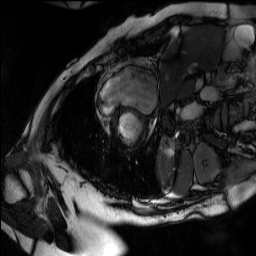
\includegraphics[width=\textwidth]{figs/modifications/ref.png}
         \caption{Référence}
         \label{fig:ref}
     \end{subfigure}
     \hfill
     \begin{subfigure}[b]{0.19\textwidth}
         \centering
         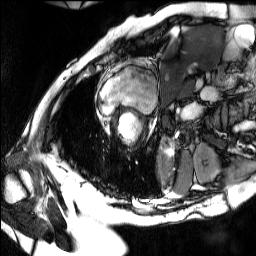
\includegraphics[width=\textwidth]{figs/modifications/contrast.png}
         \caption{Contraste}
         \label{fig:contrast}
     \end{subfigure}
	\hfill
     \begin{subfigure}[b]{0.19\textwidth}
         \centering
         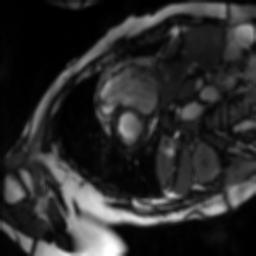
\includegraphics[width=\textwidth]{figs/modifications/blur5.png}
         \caption{Flou}
         \label{fig:blur}
     \end{subfigure}
    \hfill
     \begin{subfigure}[b]{0.19\textwidth}
         \centering
         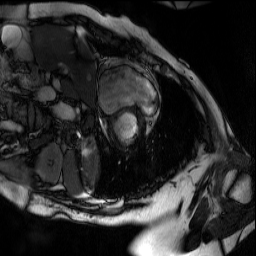
\includegraphics[width=\textwidth]{figs/modifications/hori.png}
         \caption{Miroir horizontal}
         \label{fig:hori}
     \end{subfigure}
     \hfill
	 \begin{subfigure}[b]{0.19\textwidth}
         \centering
         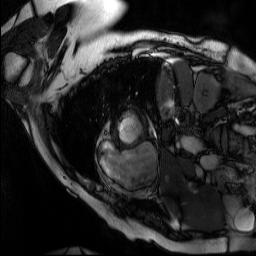
\includegraphics[width=\textwidth]{figs/modifications/vert.png}
         \caption{Miroir vertical}
         \label{fig:vert}
     \end{subfigure}
     
        \caption{Transformations du dataset}
        \label{fig:augm}
\end{figure}


Nous avons évalué nos trois réseaux U-Net entrainés avec la perte AC de l'article sur des images ayant subi ces perturbation. Les résultats sont réunis sur le Tableau \ref{tab:augm}. Ils nous permettent de comprendre que les images du dataset sont standardisées, car une modification du contraste ou de l'orientation perturbe significativement la segmentation. Il est intéressant de noter qu'un retournement horizontal a moins d'effet qu'un retournement vertical. Nous pensons que cela est lié à la structure du coeur, quasiment symétrique par rapport à l'axe vertical. L'ajout de flou, en revanche, n'a que peu d'effet, car il ne modifie que très peu l'histogramme des valeurs et le gradient moyen local. 


\begin{table}[!h]
\centering
\begin{tabular}{|l||c|}
\hline
Perturbation & Dice Score moyen\\\hline
Aucune (référence) & 0.823 \\
Flou & 0.801 \\
Contraste & 0.620 \\
Retournement horizontal & 0.463 \\
Retournement vertical & 0.129  \\

\hline
\end{tabular}
\caption{\label{tab:augm} Dice Score obtenu avec différentes perturbations}
\end{table}



\section{Conclusion}

Dans ce projet, nous avons implémenté l'article étudié \cite{learningcontour} en considérant le plus simple des deux réseaux cités, appelé U-Net. Nous avons obtenu des segmentations visuellement cohérentes, avec un Dice Score relativement proche de celui annoncé. Nous avons vu que des perturbations des images IRM en amont pouvaient conduire à de mauvaises segmentations. \\

Plusieurs extensions pourraient prolonger notre travail. L'augmentation automatique des données de départ (en ajoutant artificiellement des perturbations) pourrait former des réseaux plus robustes et précis. Il serait également intéressant d'utiliser ces segmentations comme input d'algorithmes déterministes (contour actif avec force de ballon par exemple) pour raffiner encore le résultat.

\bibliographystyle{alpha}
\bibliography{sample}
%
%\begin{table}[!h]
%\centering
%\begin{tabular}{|l||c|c|c|r|}
%\hline
%Dataset & VoxelGrid + TV & VoxelGrid & VoxelGridCarve & VoxelGridSphericalCarve \\\hline
%Drums & 20.12 dB & 20.12 dB  & 19.32 dB & 19.72 dB\\
%Chair & 23.69 dB & 23.70 dB & 24.22 dB & 26.94 dB \\ 
%Ship & 20.65  dB & 20.66 dB & 20.25 dB &  21.91 dB\\
%Ficus & 23.86 dB & 23.85 dB & 21.90 dB & 21.66 dB\\
%HotDog &  23.79 dB &  23.75 dB & 23.45 dB & 25.99 dB  \\
%Materials &  20.98 dB &  20.99 dB & 19.715 dB & 22.41 dB \\
%Lego &   21.43 dB &  21.42 dB  & 20.72 dB & 22.94 dB \\
%Mic &  22.32 dB & 22.29 dB  & 20.63 dB & 21.62 dB\\
%\hline 
%Mean & 22.10 ± 1.41  dB & 22.10 ± 1.41 dB & 21.28 ± 1.65 dB & 22.90 ± 2.24 dB \\
%\hline\hline
%Training Time & 35 minutes & 35 minutes & 1 minute & 4 minutes \\
%\hline 
%\end{tabular}
%\caption{\label{tab:psnr}PSNR on different training methods.}
%\end{table}



%
%\begin{figure}[!h]
%\centering
%\includegraphics[width=1.\textwidth]{figs/plen_pipeline.png}
%\caption{\label{fig:plenoxel} [image source: \cite{plenoxels}] The plenoxels method is composed of four steps : (a) camera rays are extracted from training images and sampled on a sparse voxel grid ; (b) the spherical harmonics of degree 9 and opacities are computed for each sample through trilinear interpolation ; (c) the resulting colors and opacities are summed to obtain a single pixel value for each ray (d) the mean squared error loss with a total variation regularizer is back-propagated to optimize the grid}
%\end{figure}
%


\end{document}
